\documentclass[a4paper,12pt]{scrreprt}
    %% Used for changing geometry of the page
    %% Cover page text cannot overlay cover sketching/style
    %% https://ctan.org/pkg/geometry?lang=en
\usepackage{geometry}
    %% Changes language of some packages protocols
    %% e.g., when captioning images: Figure 1. -> Figura 1.
    %% https://ctan.org/pkg/babel?lang=en
\usepackage[portuguese]{babel}
    %% Used for special fonts
    %% Cannot be compiled with pdflatex
    %% https://ctan.org/pkg/fontspec?lang=en
\usepackage{fontspec}
    %% Arial FONT
    \setmainfont{Arial}
    %% More colors and color options
    %% https://ctan.org/pkg/xcolor?lang=en
    %% https://ctan.org/pkg/colortbl?lang=en
\usepackage{xcolor,colortbl}
    %% More tabular options, like dashed/dotted lines
    %% https://ctan.org/pkg/arydshln?lang=en
\usepackage{arydshln}
    %% List of acronyms
    %% https://ctan.org/pkg/nomencl?lang=en
\usepackage[intoc]{nomencl}
    %% Must be called to init nomencl environment
    \makenomenclature
    %% More images options/settings
    %% https://ctan.org/pkg/graphicx?lang=en
\usepackage{graphics}
    %% Defining subdirectories to image path enviornment
    %% \graphicspath{{sub1}{sub2}...{subN}}
    \graphicspath{{images}}

    %% used to handle cross-referencing commands in LaTeX to produce hypertext links in the document
    %% https://ctan.org/pkg/hyperref?lang=en
\usepackage{hyperref}
    %% math environments
    %% https://ctan.org/pkg/amsmath?lang=en
    
    %% settings
    \hypersetup{
        colorlinks,
        citecolor=black,
        filecolor=black,
        linkcolor=black,
        urlcolor=black
    }

\usepackage{amsmath}
    %% Defining backgrouns, used to make the cover
    %% https://ctan.org/pkg/background?lang=en
\usepackage[some]{background}
    %% Used to make drawings or complex graphics
    %% http://pgf.sourceforge.net/pgf_CVS.pdf
\usepackage{tikz}
    %% Tikz library to point operations ((x1,y1) + (x2,y2))
    \usetikzlibrary{calc}

%% code snippets
\usepackage{listings}
\usepackage{color}

\definecolor{dkgreen}{rgb}{0,0.6,0}
\definecolor{gray}{rgb}{0.5,0.5,0.5}
\definecolor{mauve}{rgb}{0.58,0,0.82}

\lstset{
    frame=tb,
    %% language=Java,
    language=SQL,
    aboveskip=3mm,
    belowskip=3mm,
    showstringspaces=false,
    columns=flexible,
    basicstyle={\small\ttfamily},
    numbers=left,
    numberstyle=\small\color{gray},
    keywordstyle=\color{blue},
    commentstyle=\color{dkgreen},
    stringstyle=\color{mauve},
    breaklines=true,
    breakatwhitespace=true,
    tabsize=3,
    moredelim=**[is][\color{blue}]{@}{@}
}

%% further RelaX definitions
\usepackage{stix}

%% Defining sfdefault font and default font for document
\renewcommand{\familydefault}{\sfdefault}

%==========================================================================
% DOCUMENT
%==========================================================================

\begin{document}

\pagenumbering{gobble}

%% Costume made cover
%% From there you can use \makecover command to build the cover
%% Blue cover color
\definecolor{titlepagecolor}{RGB}{54,95,145}

%==========================================================================
% COLORED BAR ON THE LEFT SIDE
%==========================================================================

\backgroundsetup{
    scale=1, 
    angle=0, 
    opacity=1,
    contents={
        \begin{tikzpicture}[remember picture,overlay]
            \path [fill=titlepagecolor] 
                (current page.north west) -- ($(current page.north west) + (5,0)$)
                -- ($(current page.south west) + (5,0)$)-- (current page.south west); 
            \node[color=white] at ($(current page.south west) + (3,4)$) {\bfseries {\fontsize{120}{60} \textsf{LI}}};
            \node[color=titlepagecolor] at ($(current page.south west) + (5.8,4)$) {\bfseries {\fontsize{120}{60} \textsf{4}}};
        \end{tikzpicture}
    }
}

%==========================================================================
% TITLE PAGE INFO
%==========================================================================

%% Changes values in this field to show information in the cover and back cover about your team/project


%% TITLE
\title{CDC – Consultoria de Detetives Christie}

%% AUTHORS
\author{
    Afonso Dionísio Santos (A10426) \\
  \quad
    Ana Filipa Cruz Pinto (A96862) \\
  \quad
    Carlos Humberto da Silva Ferreira (A89509) \\
  \quad
    Flávia Alexandra Silva Araújo (A96587) \\
  \quad
    Miguel Torres Carvalho (A95485)
}

%% Date

\date{\today}

%% Course
\newcommand{\Course}{Licenciatura em Engenharia Informática}

%% Department
\newcommand{\Department}{Escola de Engenharia}

%% UniName
\newcommand{\UniName}{Universidade do Minho}

%% UniPic
\newcommand{\UniPic}{
\includegraphics[scale=0.09]{images/uminho.png}}

%% University 
\newcommand{\University}{
    \begin{flushleft}
        \UniPic
    \end{flushleft}
    \textcolor{gray}{\small\textbf{\textsf{\UniName}}}\par
    \textcolor{gray!80!white}{\small{\textsf{\Department}}}\par
    \textcolor{gray!70!white}{\small{\textsf{\Course}}}
}

%% UC
\newcommand{\UC}{
    \begin{flushleft}
        \par\textcolor{titlepagecolor}{  \LARGE\textbf{\textsf{Unidade Curricular de \\ Laboratórios de Informática IV}}}
    \end{flushleft}
}

%% School Year
\newcommand{\SchoolYear}{
    \small{\textsf{Ano Letivo de 2023/2024}}}


%% Define new command to show title, author and date
\makeatletter
\let\Title\@title
\let\Author\@author
\let\Date\@date
\makeatother

%==========================================================================
% CLASSIFICATION SECTION 
%==========================================================================

%% School Year
\newcommand{\ReceptionDate}{}
%% Responsible
\newcommand{\Responsible}{}
%% Evaluation
\newcommand{\Evaluation}{}
%% Observations
\newcommand{\Observations}{}





%% MAKETEMPLATE
\newcommand{\makecover}{

%==========================================================================
% BEGIN COVER PAGE 
%==========================================================================

%% Removes page number on footer
\thispagestyle{empty}

%% No indentation 
\setlength{\parindent}{0em}

%% Put Background defined on \backgroundsetup, in this page
\BgThispage

%% Changing geometry to prevent overlay with text
%% At the end of back cover, geometry is default with \restoregeometry
\newgeometry{top=5cm,left=6cm,right=3cm,bottom=2cm}

%% builds university info defined previously
\University
\vspace{1cm}
%% builds curricular unity info defined previously
\UC
%% builds school year info defined previously
\SchoolYear

\vspace*{5cm}
%% bigger space (i think its the default one) between paragraphs 
\setlength{\parskip}{1em}

%% builds title info defined previously
\par\textbf{\textsf{\huge\Title}}
\vspace{1cm}
%% builds author(s) info defined previously
\par\Author

\vspace{0.5cm}

%% builds date info defined previously
\par\Date
\restoregeometry
\pagebreak

%==========================================================================
% END COVER PAGE 
%==========================================================================

%==========================================================================
% BEGIN BACK COVER PAGE 
%==========================================================================

%% Removes page number on footer
\thispagestyle{empty}

% Changing look of lines in tabular environment 
% Dashed -> dotted 
%% length of dashes
\setlength\dashlinedash{0.3pt}
%% space between dashes
\setlength\dashlinegap{1.5pt}
%% width of dashes
\setlength\arrayrulewidth{1.1pt}


%% This values can be changed in the preamble
\begin{flushright}
\begin{tabular}{ :p{4cm}:p{4cm}: } 
\hdashline
Data de Receção & \ReceptionDate \\ [2ex]
\hdashline
Responsável & \Responsible \\ [2ex]
\hdashline
Avalição & \Evaluation \\ [2ex]
\hdashline
Observações & \Observations \\ [7ex]
\hdashline
\end{tabular}
\end{flushright}


\vspace{9cm}
\begin{flushleft}

%% builds title info defined previously
\par\textbf{\textsf{\huge\Title}}
\vspace{1cm}
%% builds author info defined previously
\par\hspace{0.25cm}\Author

\vspace{0.5cm}

%% builds date info defined previously
\par\Date
\end{flushleft}

\pagebreak
%==========================================================================
% END BACK COVER PAGE 
%==========================================================================
}


% builds the cover
\makecover

%% smaller footer and header size
\newgeometry{top=3cm,left=3cm,right=3cm,bottom=4cm}

%==========================================================================
% BEGIN OPCIONAL DEDICATÓRIA
%==========================================================================

% \clearpage
% \begin{center}
%     \thispagestyle{empty}
%     \vspace*{\fill}
%
%     $<<$/opcional Dedicatória$>>$
%
%     \vspace*{\fill}
% \end{center}
% \clearpage

%==========================================================================
% END OPCIONAL DEDICATÓRIA
%==========================================================================

%==========================================================================
% BEGIN ABSTRACT PAGE
%==========================================================================

%% Abstract name: \Large font size, flushed left and paragraph skip before abstract content
\renewenvironment{abstract}
 {\par\noindent\textbf{\Large\abstractname}\par\bigskip}
 {}

\begin{flushleft}
\begin{abstract}
    No âmbito da UC Base de Dados, lecionada pelo regente, Professor Orlando Belo, visamos a
    realização de um projeto que consiste na modelação, desenvolvimento e implementação de um
    Sistema de Base de Dados.
    \par Tendo em consideração o tema deste ano - uma agência de detetives -, decidimos explorar
    uma agência liderada por Agatha Christie, de nome CDC - Consultoria de Detetives Christie.
    Relativamente à modelação e desenvolvimento do nosso projeto, iremos dividi-lo em partes:
    começaremos de forma abstrata, transformando os factos
    \par \textbf{Área de Aplicação}: \textcolor{red}{
        <<Identificação da Área de trabalho. Por exemplo: Desenho e arquitectura de Sistemas de Bases de Dados.>>
    }
    \par \textbf{Palavras-Chave}: \textcolor{red}{
        <<Conjunto de palavras-chave que permitirão referenciar domínios de conhecimento, tecnologias, estratégias, etc., directa ou indirectamente referidos no relatório. Por exemplo: Bases de Dados Relacionais, Gestão de Índices, JAVA, Protocolos de Comunicação.>>
    }
\end{abstract}
\end{flushleft}

\pagebreak

%==========================================================================
% END ABSTRACT PAGE
%==========================================================================

%==========================================================================
% BEGIN INDEXES PAGES
%==========================================================================

%% Changes table of content name
%% Portuguese babel default : "Conteúdo"
%% Personally I prefer "índice"
\renewcommand{\contentsname}{Índice}
\renewcommand{\listfigurename}{Índice de Figuras}
\renewcommand{\listtablename}{Índice de Tabelas}

\tableofcontents

\pagebreak

\listoffigures

\pagebreak

\listoftables

\pagebreak

%==========================================================================
% END INDEXES PAGES
%==========================================================================

%==========================================================================
% BEGIN INTRODUCTION
%==========================================================================

%% Starting page numbering here
\pagenumbering{arabic}

\chapter{Definição do Sistema}
    \section{Contexto de Aplicação}
    Agatha Christie, uma figura proeminente no mundo dos detetives, criou a sua própria agência
    no final dos anos 90 após concluir que a sua carreira como detetive privada não ia ser
    suficiente para vingar-se do mundo sujo e curioso do crime.

    \par A sua agência começou como algo discreto - um escritório na periferia de Londres,
    constituído por Agatha - gerente e secretária, a cara da Consultoria de Detetives Christie
    (CDC) - e mais três detetives, responsáveis por resolver os casos dos clientes que recorriam
    à agência nos seus momentos de aflição.
    
    \par Não obstante, nos últimos três anos, houve um crescimento exponencial de casos, visto que a
    sua agência tornou-se renomada devido a alta variedade de casos que é capaz de solucionar -
    desde os mais “mundanos”, como casos de infidelidade e perseguições, até aos mais
    “mórbidos”, como homicídios e desaparecimentos. E, visto que Agatha é fascinada pelo avanço
    tecnológico, a sua consultoria também é exemplo de vanguarda na solução de cibercrimes.
    
    \par Como tal, toda esta nova popularidade acrescida levou a que Agatha contratasse um novo
    estagiário, aumentando a sua equipa e procurando conseguir prepará-lo para a subida de
    casos que a agência enfrentava a todo o vapor.

    \par Agatha Christie decidiu contratar a SIM, uma empresa de soluções informáticas portuguesa,
    para desenvolver um sistema de gestão do seu negócio depois de ouvir falar que os portugueses
    são baratos, mas sabem inglês.

    \par A SIM - Soluções Informáticas Minho - é uma empresa de consultoria informática fundada em
    Braga em 2003 onde hoje ainda está sediada. Esta oferece serviços como o desenvolvimento e
    implementação de sistemas de bases de dados (SBD).

    \pagebreak
    

    \section{Motivação e Objetivos do Trabalho}
    A CDC enfrenta um aumento significativo na procura dos seus serviços de investigação devido à
    sua reputação crescente e à diversificação dos casos com que lida. Infelizmente, Agatha sentiu a sua
    valiosa agência a sofrer complicações a partir do momento em que decidiram aceitar um maior número
    de casos. O aumento na procura por serviços de investigação levou a uma sobrecarga nos sistemas de
    gestão de casos existentes, e os registos físicos que ela mantinha desde o início da sua
    agência não lhe permitiam atribuir com rapidez suficiente os seus detetives aos casos, e muitas das
    informações cruciais, como pistas ou relatos de testemunhas, já haviam sido perdidos ou duplicados
    no passado, o que fazia Agatha temer que a sua agência acabasse por ficar com uma má reputação.
    
    \par Com a sua mente analítica e perspicaz, ela reconheceu que a chave para resolver este mistério
    organizacional estava  na modernização tecnológica, nomeadamente, na implementação de um Sistema de
    Base de Dados que possa lidar com a crescente quantidade de informações e casos de forma eficiente e
    escalável, bem como gerenciar e organizar as informações relacionadas aos casos, clientes, evidências
    e suspeitos. Este projeto visa atender a essa demanda e proporcionar à CDC as ferramentas necessárias
    para continuar a oferecer serviços de alta qualidade e eficácia, assim garantindo o sucesso da agência
    e aliviando as preocupações de Agatha sobre a popularidade acrescida.
    
    \par Por conseguinte, os objetivos principais que pretendemos alcançar com o desenvolvimento deste SBD são os seguintes:
    
    \begin{itemize}
        \item \textbf{Escalabilidade:} À medida que a CDC cresce e enfrenta um aumento contínuo na procura pelos
            seus serviços, é essencial ter um sistema que possa escalar para atender às necessidades em constante
            evolução da agência. Um Sistema de Base de Dados escalável pode crescer junto com a CDC, garantindo que
            ela permaneça ágil e adaptável às mudanças no mercado, sem falhas ou confusões no sistema.
            
        \item \textbf{Centralização dos Dados:} Com um Sistema de Base de Dados, os dados relacionados a
            casos, clientes, evidências e investigações podem ser acedidos rapidamente num local centralizado de
            forma rápida e eficiente, o que permite uma colaboração mais eficaz entre os detetives e facilita a
            tomada de decisões informadas.
            
        \item\textbf{Eficiência Operacional:} Com o aumento do volume de casos, os métodos manuais de organização de informações tornaram-se cada vez mais ineficientes. Um Sistema de Base de Dados pode automatizar diversas tarefas, como armazenamento, recuperação e atualização de dados, libertando tempo e recursos dos funcionários para se concentrarem na própria investigação.
            
            
        \item \textbf{Precisão e Consistência:} Os registos físicos estão sujeitos a erros humanos, como duplicação e perda de dados. Um Sistema de Base de Dados garante precisão e consistência nas informações, ajudando assim a evitar erros e inconsistências que possam comprometer a qualidade do trabalho da CDC.

        \item \textbf{Segurança de dados:} Os registos físicos podem ser facilmente acedidos por qualquer pessoa
            que os encontre. Isso inclui funcionários não autorizados ou intrusos, provocando falsificações, destruição
            acidental e intencional de provas. Com a implementação de Sistema de Bases de Dados, existe um maior
            controlo de acesso.
            
        \item \textbf{Controlo de Despesas:} Com a quantidade de informação que ocorre durante um caso, alguns registos de despesas podem ser esquecidas, por isso é importante saber qual foi o custo de um caso.
    \end{itemize}
    
    \section{Análise da Viabilidade do Processo}
        A viabilidade de um projeto de desenvolvimento de software depende da habilidade de compreender e satisfazer as
        demandas do mercado e dos utilizadores. Isto requer um planeamento cuidadoso e eficiente para garantir a
        entrega de um produto confiável e de alta qualidade. E, ao seguir uma abordagem metódica, o projeto pode
        maximizar as suas chances de sucesso ao atender às expectativas e necessidades do público-alvo de forma eficaz.
        
        \par Consideramos que o desenvolvimento de um SBD para a CDC é bastante viável, pois este garantirá uma série de benefícios para a agência, nomeadamente:
        
        \begin{itemize}
            \item \textbf{Melhor Gestão de Funcionários:} Com um Sistema de Base de Dados, existe uma maior facilidade para identificar que funcionários estão ocupados ou disponíveis, possibilitando uma alocação mais rápida dos mesmos aos casos, bem como uma melhor assistência destes conforme necessária.
            
            \item \textbf{Melhor Gestão da Consultoria:} Ao conhecer os custos de cada caso, é possível otimizar os recursos financeiros, planear orçamentos mais precisos e tomar decisões estratégicas fundamentadas para maximizar a eficiência e rentabilidade da empresa.
            
            \item \textbf{Melhorar a Qualidade de Serviço e de Bem Estar no Trabalho:} Um Sistema de Bases de Dados
                promoverá um melhor bem estar aos seus funcionários, evitando buscas intensivas ao sistema de
                informação já recolhida, consequentemente melhorando a qualidade do serviço, significativamente.
                
            \item \textbf{Resolver a Sobrecarga:} Devido aos dois pontos referidos anteriormente, os funcionários
                serão capazes de resolver um caso com mais eficiência e rapidez, ficando disponíveis mais rapidamente.
                Como tal, a sua produtividade vai aumentar e vai ficar a par da nova enchente de casos.
                
            \item \textbf{Segurança Acrescida:} Com um Sistema de Base de Dados, existe um maior controlo de acesso relativamente a informações cruciais aos casos, o que garante a inexistência de adulteração ou destruição de provas. Com isto, tem-se a certeza que as informações presentes nos registos são as originais e não foram acedidas por intrusos.
        \end{itemize}
        \par Considerando esses fatores, fica claro que o projeto de implementação do Sistema de Base de Dados é
        altamente viável e trará benefícios substanciais para a CDC, principalmente a níveis financeiros, de
        organização de dados e serviços, e, a longo prazo, de crescimento contínuo no mercado de detetives particulares.
    \section{Recursos e Equipa de Trabalho}
        \subsection{Recursos Humanos:}
            \begin{itemize}
                \item Funcionários da Consultoria (Detetives, estagiários e gerente);
                \item Clientes (Vítimas e os seus familiares, etc);
                \item Equipa de desenvolvimento.
            \end{itemize}
        \subsection{Recursos Físicos:}
            \begin{itemize}
                \item Computadores;
                \item Conexão à \textit{Internet};
                \item Servidor.
            \end{itemize}
        \subsection{Recursos Digitais:}
            \begin{itemize}
                \item Sistemas Operativos: \textit{Windows} 11 e \textit{Linux} (\textit{Ubuntu} 22.04.3 \textit{LTS});
                \item \textit{Google Drive};
                \item \textit{GitHub};
                \item \textit{LaTeX};
                \item brModelo (v3.31);
                \item \textit{RelaX} (https://dbis-uibk.github.io/relax);
                \item \textcolor{red}{(...) vamos preenchendo isto à medida que vamos usando ferramentas}.
            \end{itemize}
        \subsection{Equipa de Trabalho:}
            \begin{itemize}
                \item \textbf{Perssoal Interno:}
                \begin{itemize}
                    \item \textbf{Agatha Christie:} Funcionamento da agência, atendimento a clientes,
                        validação de serviços, atribuição de casos aos agentes, depoimento de informações
                        cruciais ao projeto.
                    \item \textcolor{red}{\textbf{Detetives efetivos:}}
                    \item \textcolor{red}{\textbf{Detetives estagiários:}}
                \end{itemize}
            \item \textbf{Pessoal Externo:} \textcolor{red}{(para continuar ao longo do tempo)}
                \begin{itemize}
                    \item \textbf{Afonso Santos:}
                    \item \textbf{Ana Pinto:}
                    \item \textbf{Carlos Ferreira:} Levantamento de Requisitos
                    \item \textbf{Flávia Araújo:}
                    \item \textbf{Miguel Carvalho:} Levantamento de Requisitos
                \end{itemize}
            \end{itemize}

    \section{Plano de Execução do Projeto}
        \par Para assegurar uma implementação eficiente e eficaz do sistema de bases de dados, foram realizadas reuniões e conversas com a Sra. Christie, detetives e estagiários envolvidos no projeto. Com base nessas interações, foi estabelecido o seguinte cronograma de execução:
        \par
         \textcolor{red}{
            <<TODO: adicionar diagrama de Gantt>>
        }
        \par No cronograma referido, definimos o tempo e os intervenientes nas           várias fases do projeto.

    \section{Estrutura do Relatório}
        \textcolor{red}{
            <<Após a leitura da introdução de um relatório é "simpático" apresentar uma breve descrição daquilo que se vai encontrar nos demais capítulos do relatório.>>
        }
    Após a introdução, é pertinente fornecer uma visão geral da metodologia de trabalho e das estratégias utilizadas no levantamento e análise de requisitos. Além disso, será apresentada uma esquematização do modelo da base de dados, levando em consideração os requisitos levantados.

Esta secção do relatório destina-se a oferecer uma compreensão clara da abordagem adotada ao longo do projeto, bem como dos passos seguidos para desenvolver e implementar a solução proposta. Aqui está uma oportunidade para destacar a organização e o planeamento do trabalho, bem como a estruturação do processo de recolha e análise de requisitos.

        
        \textcolor{red}{[isto faz-se no fim]}
%==========================================================================
% END INTRODUCTION
%==========================================================================

%==========================================================================
% BEGIN LEVANTAMENTO E ANÁLISE DE REQUISITOS
%==========================================================================

\chapter{Levantamento e Análise de Requisitos}
    \section{Método de Levantamento e de Análise de Requisitos Adotado}
            O processo de definição de requisitos começa com uma reunião com a equipa para selecionar diversas estratégias de levantamento, de modo a captar toda a informação necessária para sustentar adequadamente e logicamente uma melhor esquematização e composição de requisitos. Das várias estratégias discutidas, assumimos que utilizamos estas:
            \begin{itemize}
            \item \textbf{Reuniões} presenciais ou onlines com a Sra. Christie e os seus Detetives, tanto em grupo quanto individualmente com o propósito de identificar os diversos processos operacionais que ocorrem na consultoria e classificá-los.
            \item \textit{\textbf{Emails}}, às vezes as melhores ideias podem surgir subitamente, e como os funcionários têm uma vida bastante atarefada, deste modo podemos comunicar de maneira mais ágil.
            \item \textbf{Análise de Documentação} como \textbf{artigos de jornais} sobre casos resolvidos pela consultoria, para a equipa estar mais contextualizada acerca da mesma.
            \textbf{Relatórios de casos resolvidos} são recursos escassos infelizmente, pelo que também recorremos à \textbf{leitura de entrevistas dos detetives} para uma melhor compreensão das estratégias e métodos que estes têm por hábito utilizar na sua resolução dos seus casos. Analisámos igualmente a \textbf{documentação} da própria consultoria, mais especificamente relatórios relacionados com os ganhos e custos ao longo dos anos da empresa.
            \end{itemize}
            
            \par Durante a reunião foi levantada a possibilidade de acompanhar uma investigação de perto, infelizmente foi negada por questões de segurança e de confidencialidade das informações dos participantes da investigação. 

            
    \section{Organização dos Requisitos Levantados}
        \textcolor{red}{
            >> Explicação do processo de levantamento realizado e exposição da organização de requisitos adotada. Enumeração e organização dos requisitos levantados, de acordo com a sua categorização (descrição, manipulação e controlo). Caracterização dos requisitos tendo em consideração os seguintes elementos: tipo, número, data, descrição do requisito, fonte de informação e analista.
        }
    \section{Análise e Validação Geral dos Requisitos}
        \textcolor{red}{
            >> Validação dos requisitos apresentados com os diversos intervenientes do processo. Relatar eventuais anomalias e ações corretivas desenvolvidas.
        }

%==========================================================================
% END LEVANTAMENTO E ANÁLISE DE REQUISITOS
%==========================================================================

%==========================================================================
% BEGIN MODELAÇÃO CONCEPTUAL
%==========================================================================

\chapter{Modelação Conceptual}
    \section{Apresentação da Abordagem de Modelação Realizada}
        {
            Após o levantamento dos requisitos com a informação obtida, iniciámos o processo de planeamento da estrutura da Base de Dados que almejamos implementar.
            Posto isto, começámos pela modelação conceptual do nosso projeto através da construção de um Diagrama ER, de modo a podermos visualizar como as entidades (caso, detetive, cliente, etc.) relacionar-se-iam entre si, bem como os atributos que ambos (entidades e relacionamentos) possam ter. Para a caracterização das entidades, atributos e relacionamentos nos subcapítulos seguintes, recorremos à caracterização sugerida em  \cite{DatabaseSystems} (Connolly \& Begg, 2015).
            \par 
            Para a construção do diagrama em si, recorremos à ferramenta BrModelo, que utiliza notação baseada na de Dr. Heuser (sendo esta fortemente alicerçada na notação de Peter Chen).
        }
    \section{Identificação e Caracterização das Entidades}
        Avaliando o funcionamento da agência de detetives de Agatha, concluímos que as entidades seriam caracterizadas pelo conjunto: Caso, Detetive, Evidência, Cliente, Suspeito e Testemunha.
        Para cumprir os requisitos levantados anteriormente, estas entidades possuem os seguintes atributos:
        \begin{itemize}

        \item \textbf{Caso:} Representa cada caso registado na agência, trazido por um cliente e investigado por detetives.
            \begin{itemize}
            \item\textbf{Sinónimos:} Investigação, Processo, Arquivo. 
            \item\textbf{Atributos:} ID, Descrição, Estado, Categoria, Data de Abertura, Data de Fechamento, Despesa (multivalorado, com Valor, Data e Descrição) e Pagamento (também multivalorado, com Valor, Data e Descrição).
            \end{itemize}

        \item \textbf{Detetive:} Representa cada detetive que trabalha na agência em cargo da investigação de casos.
            \begin{itemize}
            \item\textbf{Sinónimos:} Investigador, Funcionário, Agente.
            \item\textbf{Atributos:} ID, Nome, \textit{Email}, Telefone, Data de Nascimento, Morada, Salário, Data de Contratação, Data de Fim de Contratação, Efetivo, Estado e Especialidade.
            \end{itemize}

        \item \textbf{Evidência:} Representa cada evidência que os detetives encontraram sobre um caso, podendo esta ter sido fornecida por uma testemunha e/ou cliente e incriminatória a um suspeito.
            \begin{itemize}
            \item\textbf{Sinónimos:} Prova, Testemunho, Depoimento. 
            \item\textbf{Atributos:} ID, Data de Coleta, Descrição, Tipo e Arquivo.
            \end{itemize}

        \item \textbf{Cliente:} Representa cada cliente que contrata a agência com o intuito dos detetives resolverem o caso que propõe.
            \begin{itemize}
            \item\textbf{Sinónimos:} Inquirido, Consumidor.
            \item\textbf{Atributos:} ID, Nome, \textit{Email}, Telefone e Morada. 
            \end{itemize}

        \item \textbf{Suspeito:} Representa cada indivíduo considerado suspeito aquando a investigação de um caso por detetives.
            \begin{itemize}
            \item\textbf{Sinónimos:} Acusado, Culpado, Réu, Arguido. 
            \item\textbf{Atributos:} ID, Nome, \textit{Email}, Telefone, Data de Nascimento, Sexo, Morada, Descrição e Data de Registo.
            \end{itemize}

        \item \textbf{Testemunha:} Representa cada testemunha que fornece informação aos detetives aquan-do a investigação de um caso.
            \begin{itemize}
            \item\textbf{Sinónimos:} Informante, Depoente, Testificador.
            \item\textbf{Atributos:} ID, Nome, \textit{Email}, Telefone, Morada e Data de Registo.
            \end{itemize}
        \end{itemize}


    \section{Identificação e Caracterização dos Relacionamentos}
        Na nossa modelação, englobámos cinco tipos de relacionamentos entre as entidades - três dos quais originam uma entidade. Devido a estas diferenças, aprofundaremos de forma individual cada um deles neste subcapítulo.

        \begin{itemize}
        \item\textbf{Relacionamento Detetive-Caso}
        \begin{itemize}
            \item\textbf{Relacionamento:} Detetive vinculado a Caso.
            \item\textbf{Descrição:} Com o intuito de poder estabelecer as vinculações dos detetives aos casos, é importante armazenar a informação desta forma para saber que detetives estão vinculados a quais casos, e durante quanto tempo foi a sua vinculação a estes. Saberemos, deste modo, se um caso tem os detetives necessários e/ou se certos detetives estão livres para serem encaminhados para novos casos.
            \item\textbf{Multiplicidade:} Detetive (0,n) - Caso (1,n): Todos os detetives têm pelo menos zero ou mais casos vinculados, e todos os casos têm pelo menos um detetive vinculado.
            \item\textbf{Baseado nos Requisitos:}
            \begin{itemize}
                \item [R6]: "Todos os casos têm vinculados pelo menos um detetive."
                \item [R18]: "Todos os detetives têm vinculado zero ou mais casos."
                \item [R31]: "Um registo de uma vinculação efetua a ligação entre um caso e os seus detetives, e deve incluir os seguintes atributos: data de vinculação, data de desvinculação (opcional) e descrição."
            \end{itemize}
            \item\textbf{Atributos:} Data de Vinculação, Data de Desvinculação e Descrição.
            \item\textbf{Entidade Gerada:} Vinculação.
        \end{itemize}
        
        \item\textbf{Relacionamento Evidência-Caso}
        \begin{itemize}
            \item\textbf{Relacionamento:} Evidência referente a Caso
            \item\textbf{Descrição:} Visto que evidências são fatores cruciais num caso, é importante o armazenamento das informações desta maneira de forma a poder facilmente aceder a todas as evidências encontradas referentes a um caso em específico, deste modo garante-se um acesso mais eficiente à informação desejada.
            \item\textbf{Multiplicidade:} Evidência (1,1) - Caso (0,n): Uma evidência tem sempre apenas um caso associado, e um caso pode ter entre zero a várias evidências associadas.
            \item\textbf{Baseado nos Requisitos:}
            \begin{itemize}
                \item [R10]: "Todos os casos têm zero ou mais evidências."
                \item [R37]: "Todos as evidências têm associadas um único caso."
            \end{itemize}
            \item\textbf{Atributos:} Nenhum.
            \item\textbf{Entidade Gerada:} Nenhuma.
        \end{itemize}
        
        \item\textbf{Relacionamento Cliente-Caso}
        \begin{itemize}
            \item\textbf{Relacionamento:} Cliente requisita Caso.
            \item\textbf{Descrição:} Com o intuito de poder registar que clientes requisitam quais casos, toda a informação relativa à requisição dos mesmos é armazenada desta forma.
            \item\textbf{Multiplicidade:} Cliente (1,n) - Caso (1,1): Um cliente pode estar associado a vários casos, porém um caso só pode estar associado a um cliente.
            \item\textbf{Baseado nos Requisitos:}
            \begin{itemize}
                \item [R7]: "Todos os casos têm associados um único cliente."
                \item [R47]: "É permitido pelo sistema obter todos os pagamentos efetuados por um cliente em diferentes casos."
            \end{itemize}
            \item\textbf{Atributos:} Nenhum.
            \item\textbf{Entidade Gerada:} Nenhuma.   
        \end{itemize}
        
        \item\textbf{Relacionamento Caso-Suspeito}
        \begin{itemize}
            \item\textbf{Relacionamento:} Caso \textit{"CasoSuspeito"} Suspeito.
            \item\textbf{Descrição:} De forma a poder registar devidamente todos os suspeitos encontrados pelos detetives relativamente a um caso que estão a investigar, é importante armazenar a informação desta forma para tal ser feito. Assim, sempre que encontrar em uma nova pista, podem voltar a rever a sua lista de suspeitos com detalhe.
            \item\textbf{Multiplicidade:} Caso (0,n) - Suspeito (1,n): Todos os casos têm, pelo menos, zero ou mais suspeitos associados, e todos os suspeitos têm, pelo menos, um caso vinculado.
            \item\textbf{Baseado nos Requisitos:}
            \begin{itemize}
                \item [R9]: "Todos os casos têm zero ou mais suspeitos."
                \item [R30]: "Devido a natureza do relacionamento entre suspeitos e casos (N:M) é feito um mapeamento entre os identificadores de caso e de suspeito."
            \end{itemize}
            \item\textbf{Atributos:} Nenhum.
            \item\textbf{Entidade Gerada:} CasoSuspeito.
        \end{itemize}
    
        \item\textbf{Relacionamento Caso-Testemunha}
        \begin{itemize}
            \item\textbf{Relacionamento:} Caso \textit{"CasoTestemunha"} Testemunha.
            \item\textbf{Descrição:} Para garantir uma investigação eficaz, é crucial documentar organizadamente todas as testemunhas encontradas relativamente a um caso, incluindo os seus detalhes e relatos para referência futura e análise detalhada.
            \item\textbf{Multiplicidade:} Caso (0,n) - Suspeito (1,n): Todos os casos têm, pelo menos, zero ou mais testemunhas associadas, e todas as testemunhas têm, pelo menos, um caso vinculado.
            \item\textbf{Baseado nos Requisitos:}
            \begin{itemize}
                \item [R8]: "Todos os casos têm zero ou mais testemunhas."
                \item [R26]: "Devido a natureza do relacionamento entre testemunhas e casos (N:M) é feito um mapeamento entre os identificadores de caso e de testemunha."
            \end{itemize}
            \item\textbf{Atributos:} Nenhum.
            \item\textbf{Entidade Gerada:} CasoTestemunha.
        \end{itemize}
        \end{itemize}
       
    \section{Identificação e Caracterização dos Atributos das Entidades e dos Relacionamentos}
        \textcolor{red}{
            <<Explicação do processo de identificação dos vários atributos das entidades e dos relacionamentos. Enumeração e fundamentação de cada atributo, organizando-os por entidades e relacionamentos identificados, tendo em conta a caracterização sugerida em [Connolly e Begg, 2015]. Indicar os requisitos que originaram cada um dos atributos enumerados.>>
        }
    \section{Apresentação e Explicação do Diagrama ER Produzido}
        \textcolor{red}{
            <<Apresentação do diagrama concetual produzido. Explicação do seu processo de construção, tendo em conta as entidades e os relacionamentos identificados anteriormente, bem com as suas caracterizações em termos de atributos.>>
        }
        \newgeometry{top=0.5cm,left=0cm,right=0cm,bottom=0.5cm}
        \clearpage
        \begin{figure}[!ht]
            \centering
            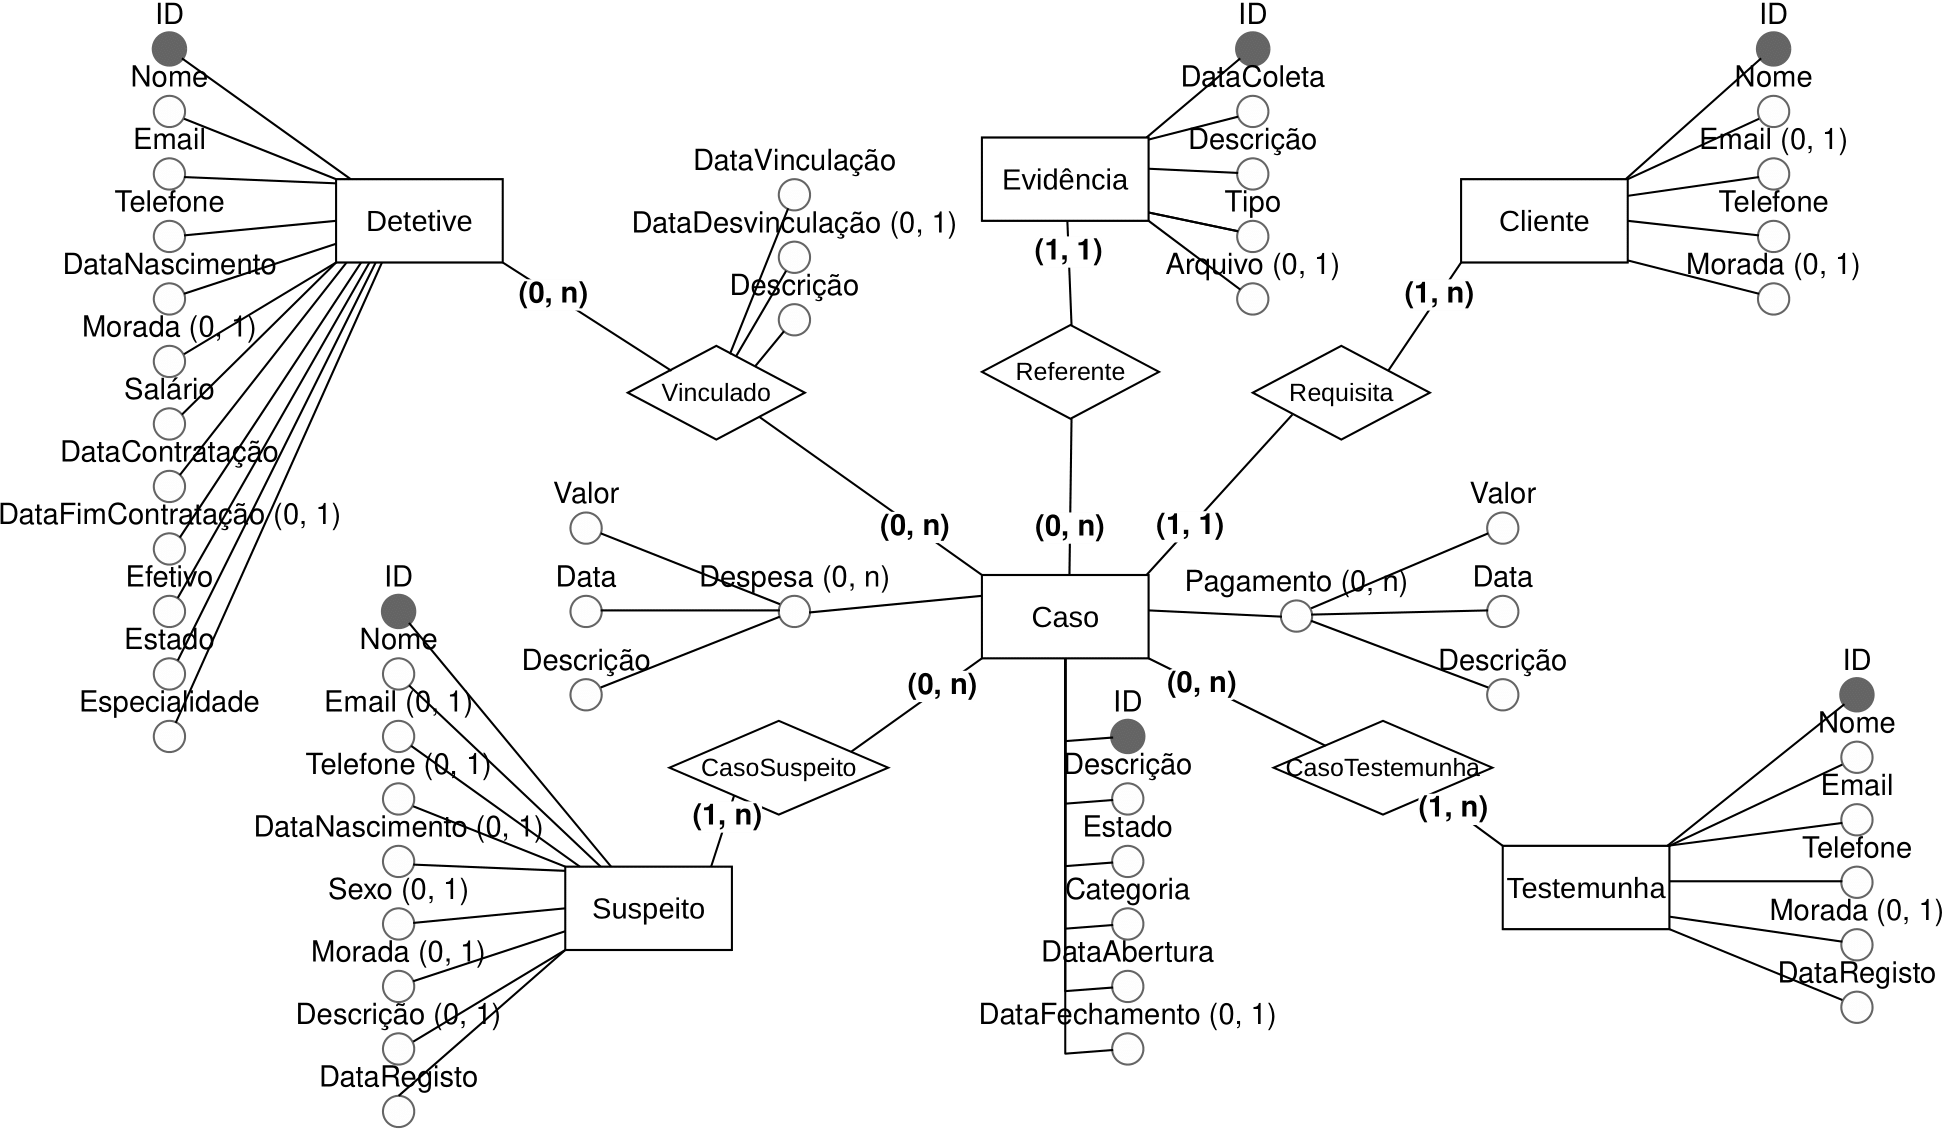
\includegraphics[scale=0.65, angle=270]{images/conceptual.png}
            \caption{Diagrama ER Conceptual}
        \end{figure}
        \newgeometry{top=3cm,left=3cm,right=3cm,bottom=4cm}

%==========================================================================
% END MODELAÇÃO CONCEPTUAL
%==========================================================================

%==========================================================================
% BEGIN MODELAÇÃO LÓGICA
%==========================================================================

\chapter{Modelação Lógica}
    \section{Construção e Validação do Modelo de Dados Lógico}
        \textcolor{red}{
            <<Apresentação e explicação do processo de modelação lógica adotado, com referência à ferramenta adotada.>>
        }
    \section{Apresentação e Explicação do Modelo Lógico Produzido}
        \textcolor{red}{
            <<Apresentação do processo de conversão realizado, expondo e justificando a origem de cada uma das tabelas que foram criadas. Apresentação do modelo lógico produzido.>>
        }
    \section{Normalização de Dados}
        De forma a garantir a normalização dos dados, é necessário considerar os seguintes pontos: \cite{DatabaseSystems} (Connolly \& Begg, 2015)
        \begin{itemize}
            \item Redução de Redundância
            \item Consistência dos Dados
            \item Facilidade de Manutenção
            \item Desempenho Aprimorado
        \end{itemize}
        O sistema de base de dados implementado visa a redução de redundância ao evitar a duplicação desnecessária de informações, proporcionando níveis de armazenamento mais económicos e evitando incongruências entre diferentes instâncias dos mesmos dados. Um exemplo da aplicação desta redução originou do relacionamento caso e suspeito, que, numa fase inicial de desenvolvimento, um suspeito estava associado a um único caso, no entanto, em um aprofundamento com os membros da CDC, concluiu-se que um suspeito tinha uma maior probabilidade de estar associado a vários casos. Após esta conclusão, o modelo foi amplificado para incluir uma relação derivada deste relacionamento, o que permite a associação de um suspeito a vários casos, evitando assim duplicações de suspeitos. O mesmo se aplicou com as entidades caso e testemunha, devido ao seu relacionamento similar ao exemplo anterior.

        Esta solução exemplificada promoveu a integridade dos dados e tornou mais fácil garantir que os dados estejam sempre corretos e atualizados, confirmando a consistência dos dados, que é fulcral à normalização destes.

        O sistema garante a facilidade de manutenção, gestão e escalonamento da plataforma, providenciando uma base ótima para estas ações, através de uma única responsabilidade para cada entidade e da organização estabelecida entre estas. Por exemplo, a criação de relações para o mapeamento de valores, tais como a categoria de um caso ou a área de especialização de um detetive, possibilita a facilidade de manutenção destes valores e endossa o escalonamento ao longo do crescimento da agência e do aperfeiçoamento na sua área de atuação.

        A plataforma demonstra padrões de centralização e padronização, permitindo aos seus utilizadores que tenham acesso às informações relevantes de forma rápida e precisa e, para além disso, a estrutura organizada do banco de dados facilita a implementação de medidas de controlo de acesso e segurança, através da definição de permissões de utilizadores específicas com base nas entidades e respetivos atributos, garantindo que apenas membros autorizados possam visualizar ou modificar determinadas informações.

        Em suma, o sistema demonstra um compromisso firme com a normalização de dados, garantindo eficiência, integridade e segurança. Ao evitar redundâncias, estabelecer relações claras entre entidades e implementar medidas de controlo de acesso, o sistema promove uma operação suave e escalável. Essa abordagem não apenas otimiza as operações atuais, mas também prepara a plataforma para um crescimento sustentável e contínuo.

    \clearpage
    \section{Validação do Modelo com Interrogações do Utilizador}
        Para assegurar a completa validade do modelo lógico de ER, foram selecionadas um conjunto de expressões algébricas derivadas dos requisitos relativos à manipulação de dados, de forma a permitirem a validação de uma grande totalidade das relações e relacionamentos estipulados no modelo. Estas serão aprofundadas nos parágrafos seguintes.

\vspace{0.5cm}
{\large 1. Aceder a identificadores de detetives que estão vinculados a um caso em específico (exemplo: ID do caso = 1), nessa instância.}

\vspace{0.2cm}
\begin{lstlisting}[escapechar=*]
*$\sigma$* (caso *$=$* 1 AND dataDesvinculacao *$=$* 'NULL') (vinculacao)
\end{lstlisting}

\begin{figure}[!ht]
    \centering
    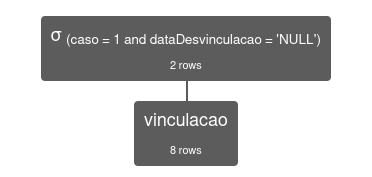
\includegraphics[scale=0.9]{images/relax/1.png}
    \caption{Representação visual da expressão em Álgebra Relacional 1.}
 \end{figure}
\vspace{0.2cm}

Esta expressão efetua uma seleção através do identificador único do caso e da data de desvinculação na entidade "vinculação" , desta forma é permitido aceder a detetives vinculados a um caso em específico nessa instância.

Ao substituir o sinal de igual pelo seu inverso em `\textit{dataDesvinculacao = 'NULL'}`, seria possível obter detetives que já estiveram vinculados ao caso, mas entretanto foram desvinculados deste.

Ao remover o termo da condição - `\textit{dataDesvinculacao = 'NULL'}` - originava uma expressão que retornava todos detetives que estão e estiveram associados a um caso em específico, ou seja todos os detetives envolvidos em um caso.

\clearpage %%\vspace{0.5cm}
{\large 2. Aceder a casos onde um detetive em específico (exemplo: ID do detetive = 1) está ativamente vinculado, nessa instância.}

\vspace{0.2cm}
\begin{lstlisting}[escapechar=*]
*$\sigma$* (detetive *$=$* 1 AND dataDesvinculacao *$=$* 'NULL') (vinculacao)
\end{lstlisting}

\begin{figure}[!ht]
    \centering
    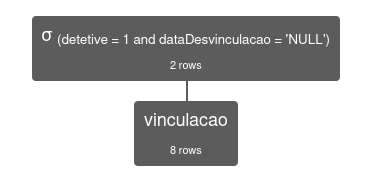
\includegraphics[scale=0.9]{images/relax/2.png}
    \caption{Representação visual da expressão em Álgebra Relacional 2.}
\end{figure}
\vspace{0.2cm}

Similarmente à expressão analisada anteriormente, é possível, através do identificador de um detetive, aceder aos casos onde este está/esteve vinculado. Neste cenário são apresentados casos onde o detetive se encontra ativamente vinculado a estes.

A obtenção de resultados conforme a atividade do detetive na investigação de um caso varia de acordo com as modificações do segundo termo da condição abordadas na primeira expressão algébrica estudada.

\clearpage %%\vspace{0.5cm}
{\large 3. Relatório completo de pagamentos com data, descrição e valor para um caso em específico (exemplo: ID do caso = 1).}

\vspace{0.2cm}
\begin{lstlisting}[escapechar=*]
*$\pi$* data, valor, descricao
*$\sigma$* (caso *$=$* 1) (pagamento)
\end{lstlisting}

\begin{figure}[!ht]
    \centering
    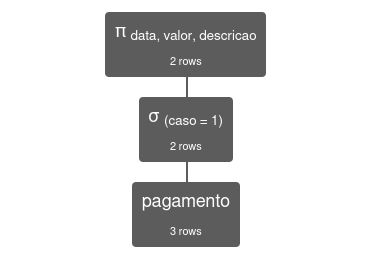
\includegraphics[scale=0.9]{images/relax/3.png}
    \caption{Representação visual da expressão em Álgebra Relacional 3.}
\end{figure}
\vspace{0.2cm}

A expressão algébrica número 3 permite a obtenção de todos os pagamentos efetuados relativos a um caso em específico, realizando uma projeção dos atributos data, valor e descrição, seguida de uma seleção da entidade "pagamento" através do identificador do caso.

Uma expressão algébrica para a obtenção de todas as despesas efetuadas relativas a um caso seria semelhante a expressão apresentada, com a diferença do acesso à entidade "despesa" em vez de "pagamento", isto deve-se a conveniente similaridade dos atributos dessas entidades. 

\clearpage %%\vspace{0.5cm}
{\large 4. Estatísticas de casos abertos, fechados e arquivados numa semana específica (exemplo: de 12/03/2024 a 18/03/2024).}

\vspace{0.2cm}
\begin{lstlisting}[escapechar=*]
*$\pi$* caso.id, caso.dataAbertura, casoestado.designacao
((*$\sigma$* (dataAbertura *$\geq$* '14/03/2024' AND dataAbertura *$\leq$* '20/04/2024') (caso))
*$\bowtie$* caso.estado *$=$* casoestado.id (casoestado))
\end{lstlisting}

\begin{figure}[!ht]
    \centering
    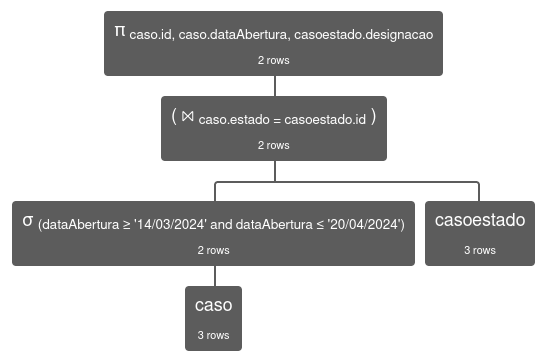
\includegraphics[scale=0.77]{images/relax/4.png}
    \caption{Representação visual da expressão em Álgebra Relacional 4.}
\end{figure}
\vspace{0.2cm}

A expressão algébrica número 4 obtém os identificadores de casos e o seu respetivo estado atual, onde estes são inicializados numa determinada semana. Esta serve para demonstrar o uso de entidades de mapeamento de valores, que, neste caso, foi utilizada a entidade "casoestado" para mapear o atributo estado de um caso, representado por um número inteiro com a sua respetiva designação ("aberto", "fechado" ou "arquivado").

Uma otimização possível a esta expressão seria a truncação dos atributos \textit{id} e \textit{dataAbertura} da entidade "caso" antes da seleção através da data de abertura, desta forma, era aumentada a eficiência da expressão. A equipa de trabalho decidiu não incluir esta otimização de forma a manter a simplificação da expressão algébrica apresentada. 

\clearpage %%\vspace{0.5cm}
{\large 5. Apresentar os dados de um caso (exemplo: ID do caso = 1) - evidências, suspeitos e testemunhas - por ordem cronológica.}

\vspace{0.2cm}
\begin{lstlisting}[escapechar=*]
-- a) Obter todas as evidências relativas a um caso por ordem cronológica
*$\tau$* evidencia.dataColeta ASC
*$\sigma$* (caso *$=$* 1) (evidencia)

-- b) Obter todos os suspeitos relativos a um caso por ordem cronológica
*$\tau$* suspeito.dataRegisto ASC
*$\pi$* suspeito.nome, suspeito.telefone, suspeito.email, suspeito.dataNascimento, suspeito.sexo, suspeito.morada, suspeito.descricao, suspeito.dataRegisto
(*$\sigma$* (casosuspeito.caso *$=$* 1) (casosuspeito)
*$\bowtie$* casosuspeito.suspeito *$=$* suspeito.id (suspeito))

-- c) Obter todas as testemunhas relativas a um caso por ordem cronológica
*$\tau$* testemunha.dataRegisto ASC
*$\pi$* testemunha.nome, testemunha.telefone, testemunha.email, testemunha.morada, testemunha.dataRegisto
(*$\sigma$* (casotestemunha.caso *$=$* 1) (casotestemunha)
*$\bowtie$* casotestemunha.testemunha *$=$* testemunha.id (testemunha))
\end{lstlisting}

\begin{figure}[!ht]
    \centering
    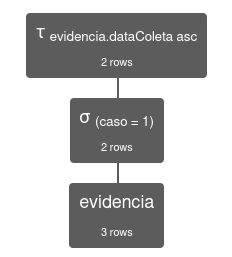
\includegraphics[scale=0.9]{images/relax/5-a.png}
    \caption{Representação visual da expressão em Álgebra Relacional 5.a)}
\end{figure}

\clearpage

\begin{figure}[!ht]
    \centering
    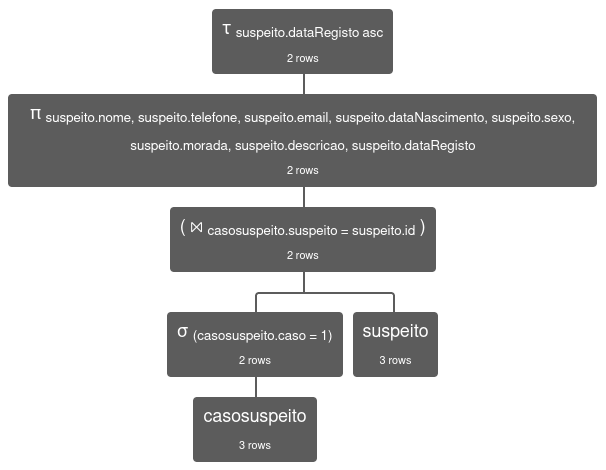
\includegraphics[scale=0.7]{images/relax/5-b.png}
    \caption{Representação visual da expressão em Álgebra Relacional 5.b)}
\end{figure}

\clearpage

\begin{figure}[!ht]
    \centering
    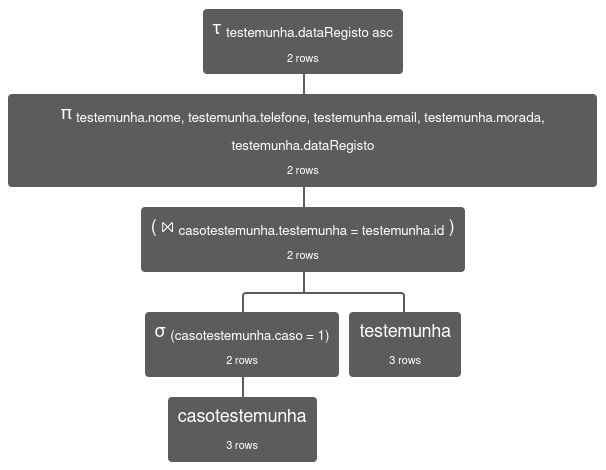
\includegraphics[scale=0.65]{images/relax/5-c.png}
    \caption{Representação visual da expressão em Álgebra Relacional 5.c)}
\end{figure}

Para apresentar os dados relativos a um caso em específico por ordem cronológica, as expressões foram divididas em três partes - a, b e c, respetivamente.

A primeira expressão (a) (figura 4.5) é responsável por apresentar todos os registos de evidências relativo a um caso, através da seleção do identificador do caso. De seguida efetua-se a ordenação crescente pela data de coleta de evidência, de forma a garantir a ordem cronológica das evidências apresentadas.

Seguidamente, a expressão (b) (figura 4.6) apresenta os dados das testemunhas de um determinado caso. Esta faz uma seleção através do identificador no caso na entidade "casotestemunha", obtendo assim todos os identificadores das testemunhas em questão. Após a truncação dos atributos relevantes às testemunhas, é feito a sua ordenação de forma crescente, através do atributo data de registo das testemunhas.

Por fim, a expressão (c) (figura 4.7) apresenta os dados dos suspeitos de um determinado caso, similarmente à expressão (b) abordada no parágrafo anterior.

Seria possível a combinação das três expressões abordadas anteriormente de forma a obter uma única tabela como resultado. Para tal, era necessário unir as expressões anteriores e renomear os atributos \textit{testemunha.dataRegisto}, \textit{suspeito.dataRegisto} e \textit{evidencia.dataColeta} para um só para a reorganização dos registos através deste novo atributo unificado.

\clearpage %%\vspace{0.5cm}
{\large 6. Relatório diário de novas evidências, suspeitos e testemunhas de um caso em específico (exemplo: ID do caso = 1 e data = 20/03/2024).}

\vspace{0.2cm}
\begin{lstlisting}[escapechar=*]
-- a) Obter as novas evidências relativas a um caso
*$\pi$* evidencia.id, evidencia.dataColeta, evidencia.descricao
*$\sigma$* (caso *$=$* 1 AND dataColeta *$=$* '20/03/2024') (evidencia)

-- b) Obter os novos suspeitos relativos a um caso
*$\pi$* suspeito.nome, suspeito.telefone, suspeito.email, suspeito.dataNascimento, suspeito.sexo, suspeito.morada, suspeito.descricao, suspeito.dataRegisto
*$\sigma$* (casosuspeito.caso *$=$* 1 AND suspeito.dataRegisto *$=$* '20/03/2024')
(casosuspeito *$\bowtie$* casosuspeito.suspeito *$=$* suspeito.id (suspeito))

-- c) Obter as novas testemunhas relativas a um caso
*$\pi$* testemunha.nome, testemunha.telefone, testemunha.email, testemunha.morada, testemunha.dataRegisto
*$\sigma$* (casotestemunha.caso *$=$* 1 AND testemunha.dataRegisto *$=$* '20/03/2024')
(casotestemunha *$\bowtie$* casotestemunha.testemunha *$=$* testemunha.id (testemunha))
\end{lstlisting}

\begin{figure}[!ht]
    \centering
    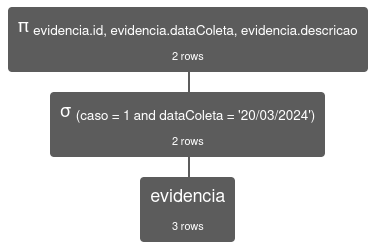
\includegraphics[scale=0.9]{images/relax/6-a.png}
    \caption{Representação visual da expressão em Álgebra Relacional 6.a)}
\end{figure}

Similarmente à interrogação anterior (5), esta foi dividida em três expressões algébricas, onde, em vez de uma ordenação cronológica, são apresentados dados através da seleção da data de coleta/registo relativa a cada entidade (evidências, suspeitos e testemunhas).

De modo semelhante à combinação descrita anteriormente, estas três expressões poderiam ser unificadas de forma a apresentar uma única tabela como resultado, através da operação $\fullouterjoin$ - "\textit{full outer join}".

\begin{figure}[!ht]
    \centering
    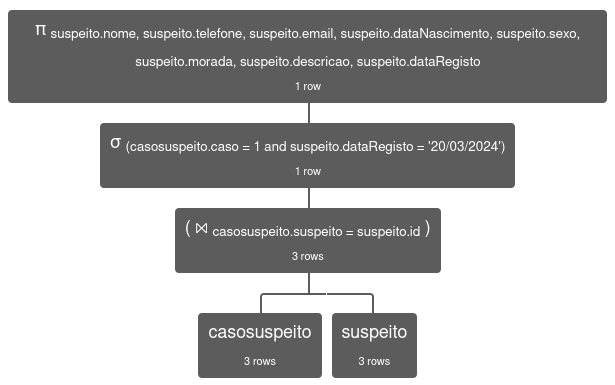
\includegraphics[scale=0.692]{images/relax/6-b.png}
    \caption{Representação visual da expressão em Álgebra Relacional 6.b)}
\end{figure}
\vspace{0cm}
\begin{figure}[!ht]
    \centering
    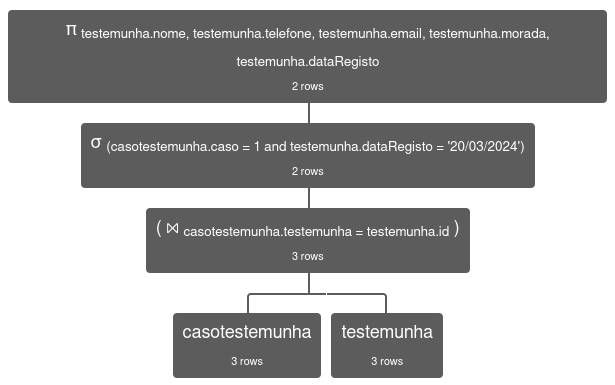
\includegraphics[scale=0.692]{images/relax/6-c.png}
    \caption{Representação visual da expressão em Álgebra Relacional 6.c)}
\end{figure}

%==========================================================================
% END MODELAÇÃO LÓGICA
%==========================================================================

%==========================================================================
% BEGIN CONCLUSÕES DE TRABALHO FUTURO
%==========================================================================

\chapter{Conclusões e Trabalho Futuro}
    \textcolor{red}{
        <<Elaborar uma apreciação crítica sobre o trabalho realizado, apontando os seus pontos fortes e fracos. Adicionalmente, caso se aplique, enunciar eventuais tarefas a realizar futuramente ou novas opções para estender o trabalho realizado.>> \\
        <<Resumo breve do trabalho realizado e das ações desenvolvidas. Enumeração e análise de aspetos positivos e negativos identificados durante o processo de desenvolvimento do sistema de bases de dados. Exposição das próximas linhas de desenvolvimento do projeto.>>
    }

    \textcolor{red}{
        <<Aqui podemos falar da entidade comunicações que não implementamos devido a sua natureza complexa e as vantagens que esta poderia trazer ao SBD>>
    }

%==========================================================================
% END CONCLUSÕES DE TRABALHO FUTURO
%==========================================================================

%==========================================================================
% BEGIN BIBLIOGRAFIA
%==========================================================================

%% Changes biblibography name
%% Portuguese babel default : "Bibliografia"
%% Personally I prefer "Referências"
% \renewcommand\bibname{Referências}

%% https://www.overleaf.com/learn/latex/bibliography_management_with_bibtex
\begin{thebibliography}{9}
\bibitem{DatabaseSystems}
Connolly, T., \& Begg, C. (2015). Database Systems: A Practical Approach to Design, Implementation, and Management (6th ed.). Pearson Education. London, UK.
\bibitem{Aprendizagem em Banco de Dados}
Carlos Henrique Cândido
\end{thebibliography}

%==========================================================================
% END BIBLIOGRAFIA
%==========================================================================

%==========================================================================
% BEGIN LISTA DE SIGLAS E ACRÓNIMOS
%==========================================================================

%% Portuguese babel does not translate this environment
\renewcommand{\nomname}{Lista de Siglas e Acrónimos}

%% Text that can be shown before acronyms list
% \renewcommand{\nompreamble}{
%     \textcolor{red}{
%         <<Apresentar uma lista com todas as siglas e acrónimos utilizados durante a realização do trabalho. O formato base para esta lista deverá ser da forma como abaixo se apresenta.>>
%     }
% }

%% acronyms
\nomenclature[01]{\textbf{CDC}}{Consultoria de Detetives Christie}
\nomenclature[02]{\textbf{SIM}}{Soluções Informáticas Minho}
\nomenclature[03]{\textbf{BD}}{Base de Dados}
\nomenclature[06]{\textbf{ER}}{Entidade-Relacionamento}
\nomenclature[04]{\textbf{SBD}}{Sistema de Base de Dados}
\nomenclature[05]{\textbf{ER}}{Entidade-Relacionamento}
\nomenclature[06]{\textbf{ID}}{Identificador}

%% Show acronyms
\printnomenclature

%==========================================================================
% END LISTA DE SIGLAS E ACRÓNIMOS
%==========================================================================

%==========================================================================
% BEGIN ANEXOS
%==========================================================================

%% Why \addchap, instead of \chapter?
%% \addchap has no numbering but appears in table of contents.
\addchap{Anexos}

    \textcolor{red}{
        <<Os anexos deverão ser utilizados para a inclusão de informação adicional necessária para uma melhor compreensão do relatório o para complementar tópicos, secções ou assuntos abordados. Os anexos criados deverão ser numerados e possuir uma designação. Estes dados permitirão complementar o Índice geral do relatório relativamente à enumeração e apresentação dos diversos anexos.>>
    }

    %% section version of \addchap
    \addsec{Anexo 1}


%==========================================================================
% END ANEXOS
%==========================================================================
\end{document}

